\chapter{Development}
\section{Application Architecture}
\label{sec:architecture}
All the iOS applications follow the model view controller architecture. This
artchitecture separates the data model ---inside the \emph{model}---, the presentation
of the data ---the \emph{view}--- and the interaction and logic between them ---the
\emph{controller}---. 

First of all we're going to discuss how Ponster applies the MVC
architecture; then we will introduce the selected persistency layer with CoreData
and finally how the augmented reality fits into the app.

\subsection{Model View Controller}
Each of the main components of Ponster is represented by a subclass of UIKit's
controller, the \texttt{UIViewController}. When developing complex applications is
frequent to have a base view controller with shared functionality. Then, the rest of
the view controllers inherit from them. In Ponster, the main view controller from
where our controllers inherit from are the ones presented by UIKit, without any
other feature added. 

We can separate the view controllers in our app with the following list:
\begin{itemize}
\item Main screen view controller.
\begin{itemize}
\item Collection view controller.
\end{itemize}
\item Poster view controller
\item Augmented reality view controller.
\end{itemize}

There is one view controller that is built from two view controllers, the main
screen. It is common in iOS to represent tables or collection views using the UIKit
view controller that is ready for those tasks, \texttt{UITableViewController} or
\texttt{UICollectionViewController}. Usually this is done because both view
controllers have built-in methods like the refresh control that are easier and
more correct to use when subclassing from those UIKit view controllers. In order to
customize the rest of the view controller and to keep responsability separated ---one
view manages the collection, the other the whole screen--- we use
view controller containment to embed the collection VC inside the main screen view
controller. This allows us to keep the single responsibility principle and to have
lighter view controllers.

Apart of the view controllers, all the data model is separated into
\texttt{NSManagedObject} subclasses. Each of that subclass represent an entity in
our model. Business logic is usually implemented as a category of each of the model
subclass. Categories in Objective-C are capable of adding methods to any object
without having to change it's implementations. This logic is usually added as a
category in order to not interfere with the \texttt{NSManagedObject} subclass,
because every time a change is made to a model, we have to generate the subclass
again and this would erase all the logic that we could have built inside.

We do not have a lot of custom views in Ponster, but we do have cell subclasses to
represent each poster in the main screen view controller. The
\texttt{UICollectionViewCell} subclass called \texttt{PNSPosterCollectionViewCell}
encapsulates all the views that are needed to display the poster image and it's
title. We just need to provide the \texttt{Poster} entity and this subclass manages
to draw the entire view.

\subsection{Persistency layer architecture}
In order to deliver a good user experience, we have to understand the iOS
architecture. iOS has a high-priority thread called \emph{Main Thread} where all the
UIKit operations must be executed. Thanks to this, the responsiveness of every UI
has the top execution priority, but it also has downsides. If our code is blocking
the Main Thread, it will also block the user interface, thus delivering a poor user
experience. To solve this potential issue, we have to send all the possible
operations to another threads.

When using a CoreData model, it is a good idea to create different
\texttt{NSManagedObjectContext}s in order to have contexts using background threads
and one context tied to the UI code to provide the views with the database
objects. If we send all the saves to the background queue, the risk of blocking the
Main Thread is reduced. Our proposed CoreData architecture~\cite{coredataarch} has
one \emph{background} context attached to the persistent store, another one attached
to the Main Thread to use it when providing data to our views and several background
contexts to perform saves.

\begin{figure}
\centering
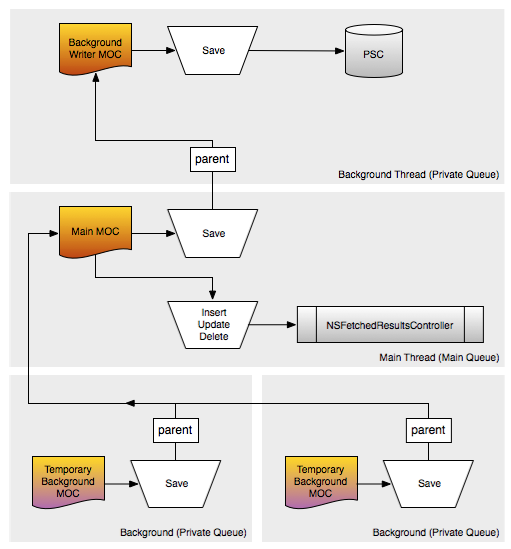
\includegraphics[scale=0.55]{img/coredataarch.png}
\caption{\label{fig:coredataarch}CoreData context architecture. Taken
  from~\cite{coredataarch}} 
\end{figure} 

The context attached to the persistent store saves all the data on disk, but on a
background thread, so the UI is never blocked. Then, all the save contexts that we
can create use a background thread and trigger the Main Thread, UI-context when they
have saved any info. This architecture is often known as \emph{child-context},
because there is a parent-child relationship between all the
contexts~\ref{fig:coredataarch}. 

\section{Augmented reality performance}
During the development of Ponster, both OpenCV and Vuforia have been tested. Due to
the low performance of OpenCV on the mobile device, Vuforia has been the chosen library
to bring the augmented reality to our app. In the performance
chart~\ref{fig:performance} we can find the average time to analyze each frame with
the different technologies tested. 

All of these tests have been executed with the iPhone 5 mobile device using iOS
8. The selected pattern to test the matching is the famous image of Lena Söderberg,
which is widely used when testing computer vision algorithms. The test consists on
running the algorithm against the Lena image while moving and rotating the camera
for a minute.

\begin{figure}
\centering
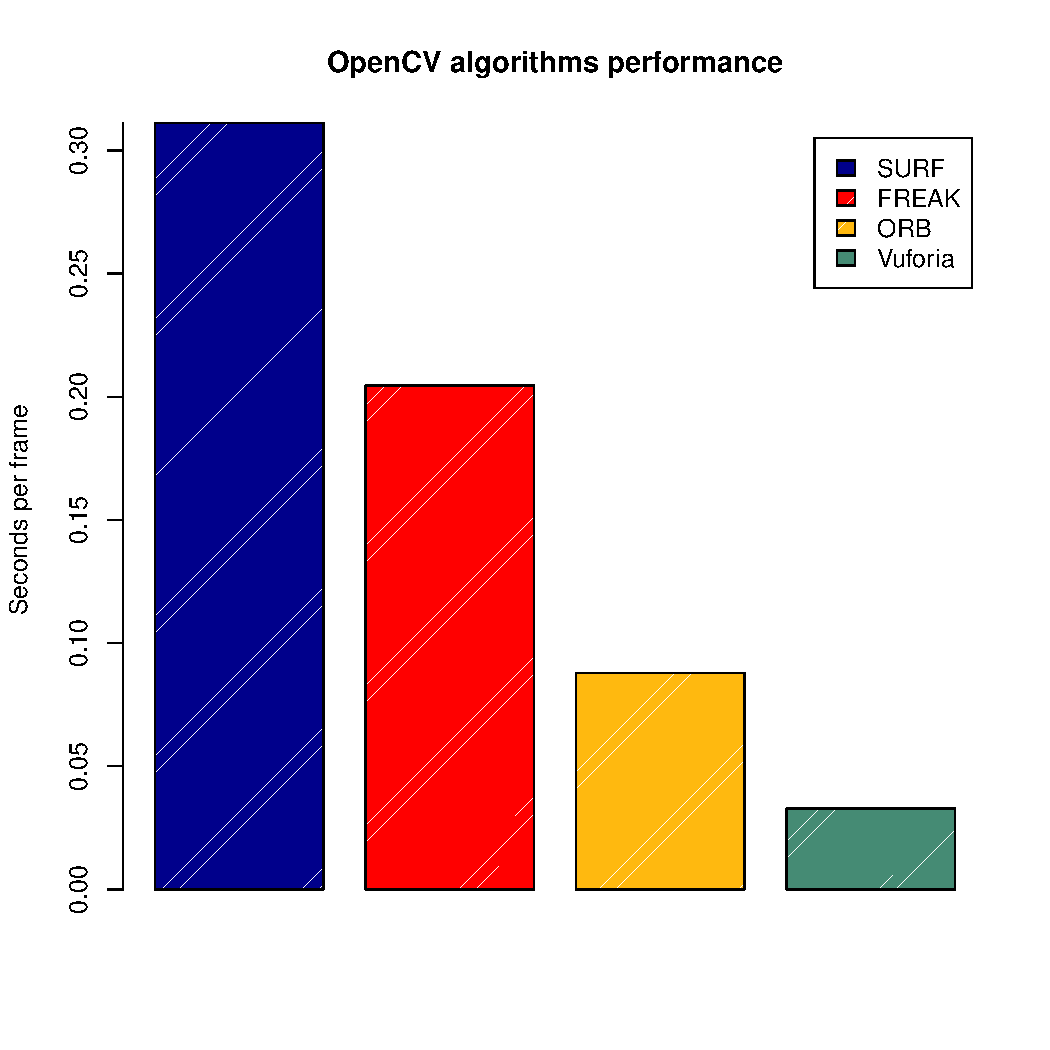
\includegraphics[scale=0.75]{performance/plot.pdf}
\caption{\label{fig:performance} Mean time spent for processing each frame with the
  different algorithms tested.}
\end{figure} 

As we can see, SURF is, by far, the most expensive technique tested on the device. This is the
expected behaviour, as it's stated in the cited articles in
section~\ref{chap:sota}. FREAK uses SURF to compute 
the keypoints, so the performance boost happens on the descriptor calculation
only. Between all the OpenCV algorithms tested, ORB is the one that performs better
while providing almost the same robustness as the other two algorithms tested.
However, the only technique that led to a real-time performance has been the Vuforia
SDK. The average frames per second of the processing with Vuforia is between 29 and
30 FPS, while maintaining the best robustness and tracking of all the above
algorithms tested. This is due to the natural feature~\ref{sec:naturalfeature}
approximation of Vuforia.

The reason behind testing only SURF, FREAK and ORB under OpenCV is that they
represent different approaches to the same problem of object tracking. Analyzing
each part of the feature detection process can bring some light to know which step
is the most expensive in terms of computational cost. In the
figure~\ref{fig:kpperformance} we can see the average time spent in each frame when
computing the keypoints with SURF and ORB detectors. FREAK has been tested with SURF
keypoint detection, so we can clearly see that the descriptor extraction by FREAK is
much more efficient than the SURF extraction.

\begin{figure}
\centering
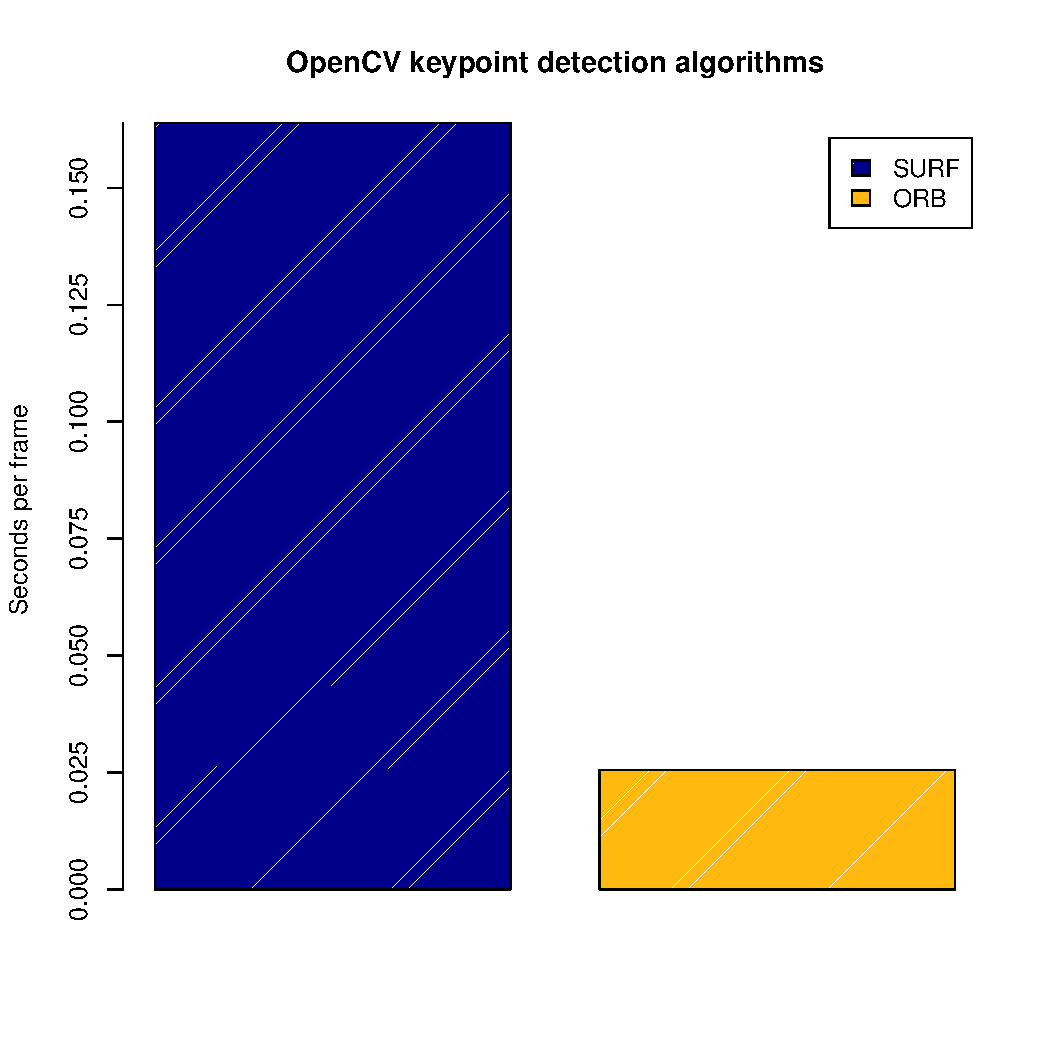
\includegraphics[scale=0.75]{performance/keypoints.pdf}
\caption{\label{fig:kpperformance} Mean time spent for detecting each frame
  keypoints with SURF and ORB.}
\end{figure} 

The number of keypoints detected between SURF and ORB is also quite different. In
the figure~\ref{fig:numberkp} we can see the average number of keypoint detected for
each frame. It is interesting to see that while ORB detects around 60\% of the
keypoints detected by SURF, it performs almost as good as SURF in terms of
robustness when detecting the selected pattern. However, while executing both
algorithms in the app, the detection of the pattern is less prone to error with
blurred or translated image using the SURF keypoint and descriptor combination. 

\begin{figure}
\centering
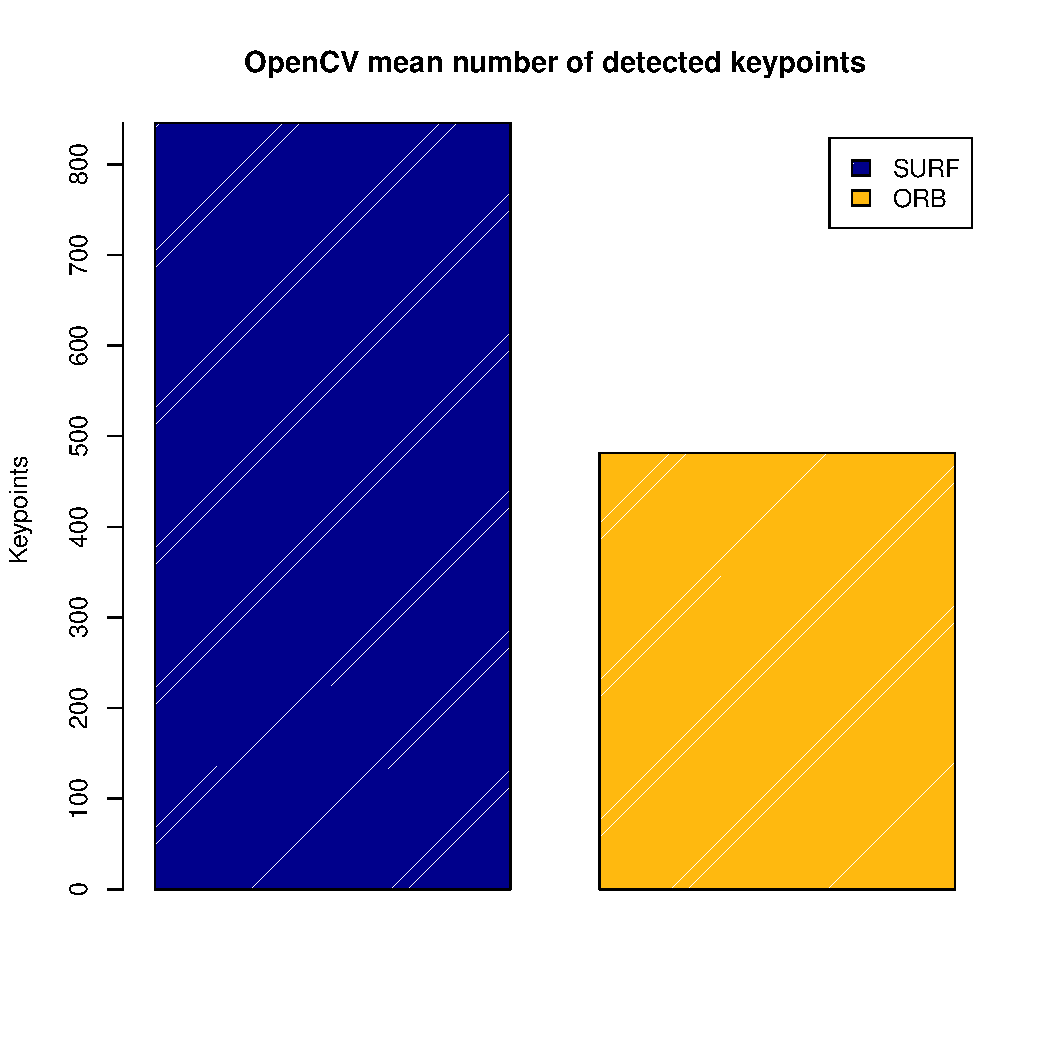
\includegraphics[scale=0.75]{performance/keypoints-number.pdf}
\caption{\label{fig:numberkp} Average number of keypoints detected using SURF and
  ORB keypoint detection algorithms.}
\end{figure} 

Finally, when we have extracted the descriptors of the image from the camera, we
have to match them with the descriptors obtained from the pattern image. Once the
match is performed, we have to calculate the homography to locate the object in the
image. Then, we can get the corners of the pattern and calculate the perspective
transform in order to draw the poster above the detected image. 

In the figure~\ref{fig:goodmatches} we can see that the SURF and Flann-based matcher
combination is the one that produces more matches, but it's also the more expensive
in terms of computational cost. SURF keypoint detector with FREAK descriptors
perform faster than the SURF approximation, but it also has lower precision when
detecting the pattern. Finally, ORB and Flann with Locality-Sensitive Hashing
parameters for the matching is the one that outperforms the previous techniques and
delivers an average number of matches similar to SURF.

\begin{figure}
\centering
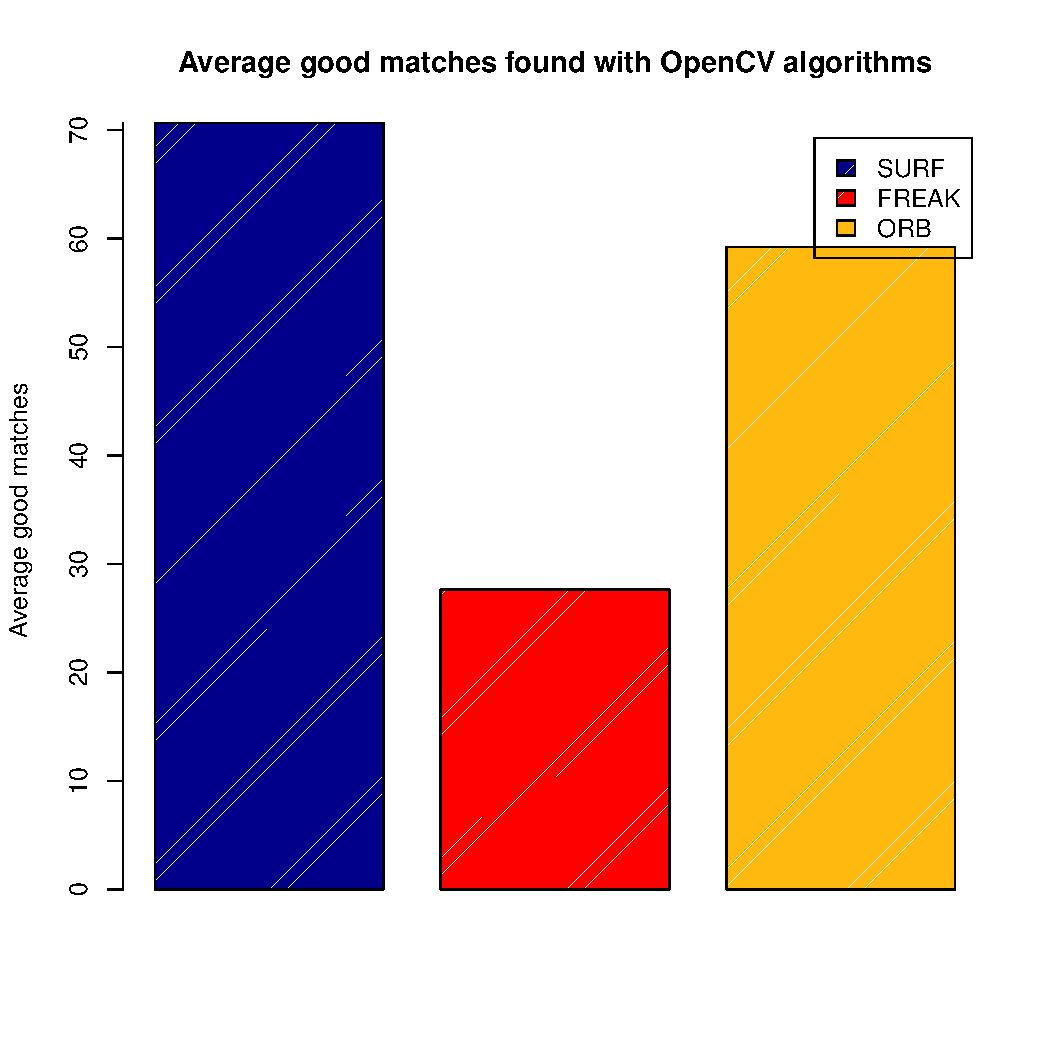
\includegraphics[scale=0.75]{performance/goodmatches.pdf}
\caption{\label{fig:goodmatches} Average number of good matches detected using the
  different algorithm and matcher combinations.}
\end{figure} 

As we have stated before, Vuforia is a propietary SDK based on natural feature
detection, and we do not have access to how it detects the pattern. This is the
reason why it is only shown in the figure~\ref{fig:performance}, because we can
estimate the time spent processing for each frame delivered by the camera.

\section{Features}
The Ponster app has three main features: list posters, try how they look wherever
the user wants and capture an screenshot of the poster in the scene.

\begin{description}
\item [List posters] \hfill \\
\item [Augmented reality] \hfill \\
\item [Screenshot] \hfill \\
\end{description}
